\documentclass{article}
\usepackage{ae,lmodern}
\usepackage[francais]{babel}
\usepackage[utf8]{inputenc}
\usepackage[T1]{fontenc}
\usepackage{graphicx}
\usepackage{float}
\usepackage{verbatim}

\title{M1 Informatique - UE ARF.\\Rapport des TME.}
\author{Treü Marc, Karmim Yannis\\Spécialité DAC.}

\begin{document}

\maketitle
\clearpage
\tableofcontents
\clearpage
Pour une meilleure lisibilité tout nos morceaux de codes pertinents se trouvent en annexe. 
\section{TME 1 : Arbres de décision, sélection de modèles.}
Sur ce TME on a travaillé sur les arbres de décision et la classification à partir de la IMDB.\\
On a dû étudier comment fonctionne ces arbres, en particulier la façon dont on les génère et on choisi nos variables de décisions à l'aide de l'entropie. Puis on a étudié les impacts des hyper-paramètres sur le taux d'erreur en apprentissage et en test pour évaluer le sur et sous apprentissage. \\
Enfin on a implémenté de la validation croisé pour calibrer ce sur-sous apprentissage.\\

\subsection{Quelques expériences préliminaires.}

\begin{figure}[h]
	\center
	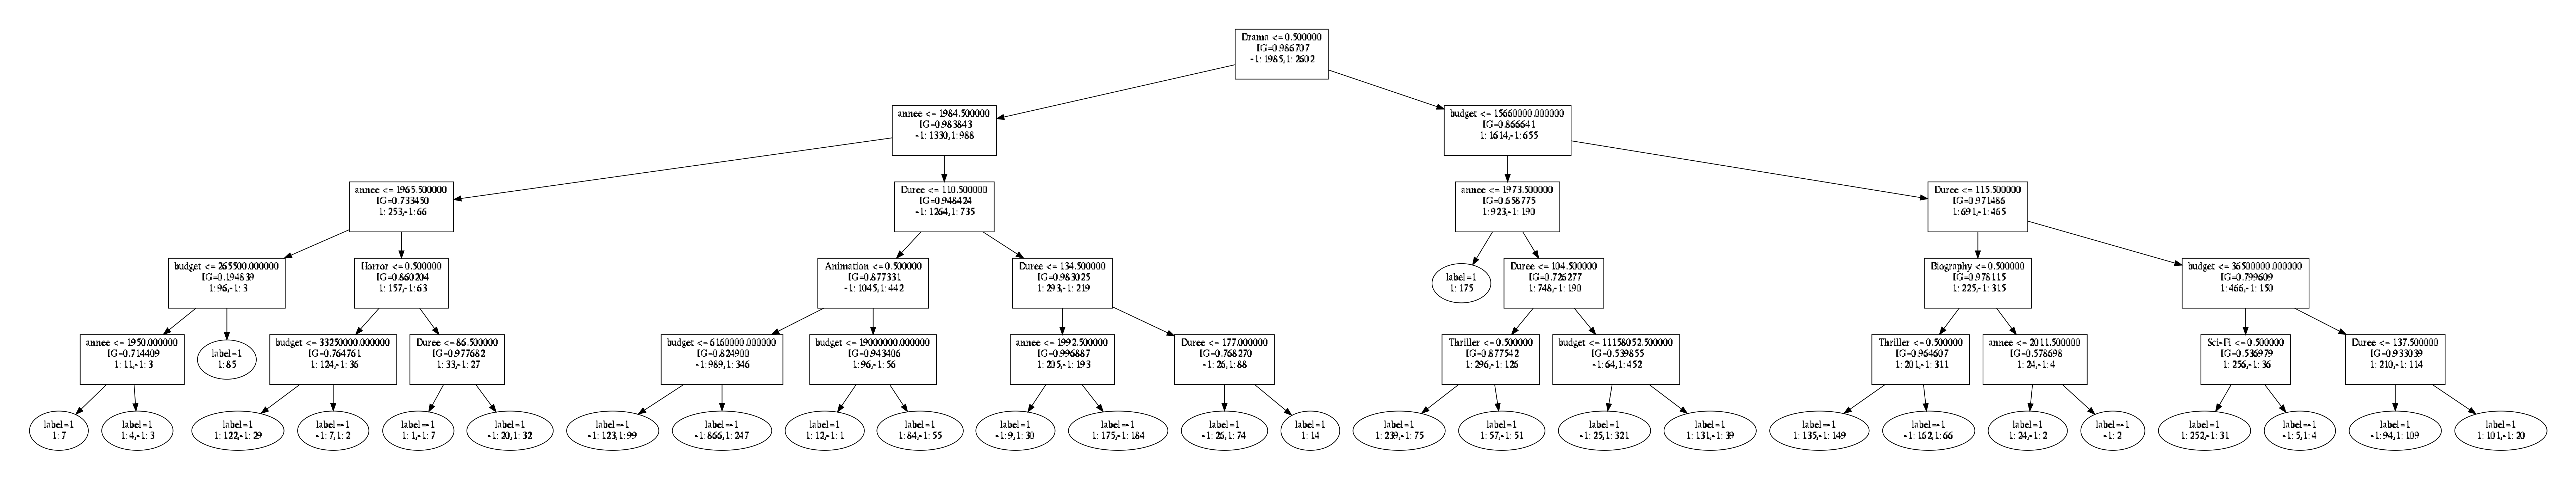
\includegraphics[width=16cm]{../tme1/test_tree.png} 
	 \caption{Exemple d'arbre généré à l'aide du code fourni et de pydot, de profondeur 5 et de score 73\% de bonne classification en apprentissage }
	 
\end{figure}
Plus on descend dans un arbre de décision moins il y a d'exemples à séparer dans les noeuds . Ce qui est normal puisque à chaque noeud de notre arbre, on divise notre base d'exemples à l'aide des critères de décision des noeuds supérieurs.\\
Si l'on test uniquement sur nos données d'apprentissage, on remarque que lorsqu'on augmente la profondeur, les scores de bonnes classifications augmentent.\\
$profondeur = 5$ : 73.6\% de bonne classification.\\
$profondeur = 15$ : 88.2\% de bonne classification.\\
$profondeur = 20$ : 89.8\% de bonne classification.\\

C'est normal que ces scores augmentent puisque notre arbre de décision tend à s'adapter parfaitement à nos données d'apprentissage. Mais il faut être vigilant au sur-apprentissage. Donc le score sur les données d'apprentissage n'est pas un indicateur fiable du comportement.\\
Il faut alors tester notre modèle sur des données que l'on a pas encore vu, on peut par exemple partitionner nos données en apprentissage et en test.\\
\subsection{Sur et sous apprentissage.}
Nous avons crée une fonction de partitionnement en test et apprentissage, et avons testé ce partitionnement sur plusieurs profondeurs d'arbres.\\
Voici plusieurs graphiques montrant nos taux d'erreurs en apprentissage et en test en fonction de la profondeur de l'arbre et chaque graphique représente un partitionnement différent.\\ 
Les courbes en pointillés représentent les erreurs en test.\\
Les courbes lisse représentent les erreurs en apprentissage.

\begin{figure}[h]
	\center
	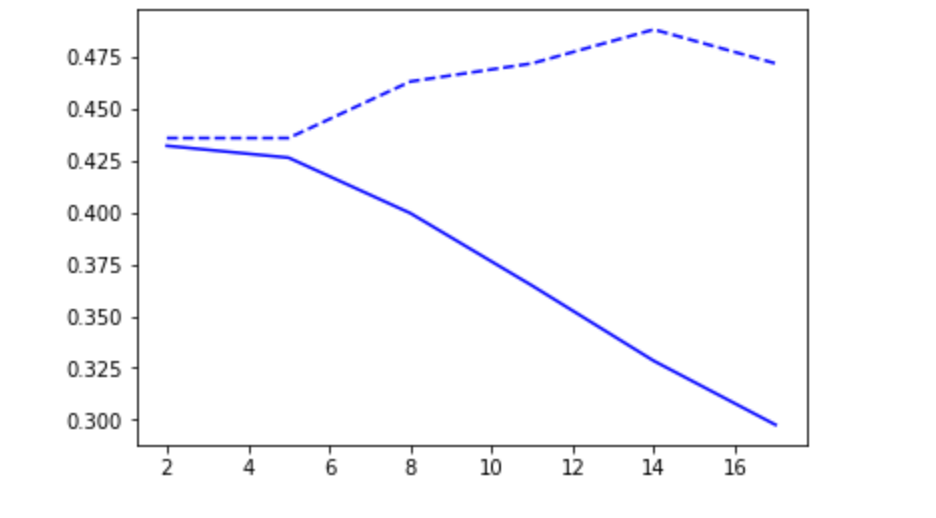
\includegraphics[width=8cm]{figure/tme1/08ap.png} 
	 \caption{Taux d'erreur en fonction de la profondeur pour un partitionnement avec 80\% des données en apprentissage }
	 
\end{figure}
\begin{figure}[h]
	\center
	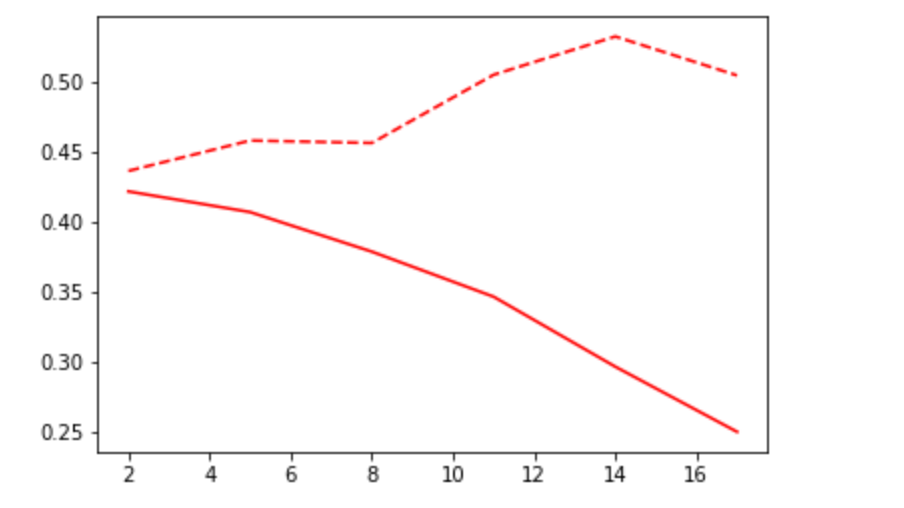
\includegraphics[width=8cm]{figure/tme1/05ap.png} 
	 \caption{Taux d'erreur en fonction de la profondeur pour un partitionnement avec 50\% des données en apprentissage }
	 
\end{figure}
\begin{figure}[h]
	\center
	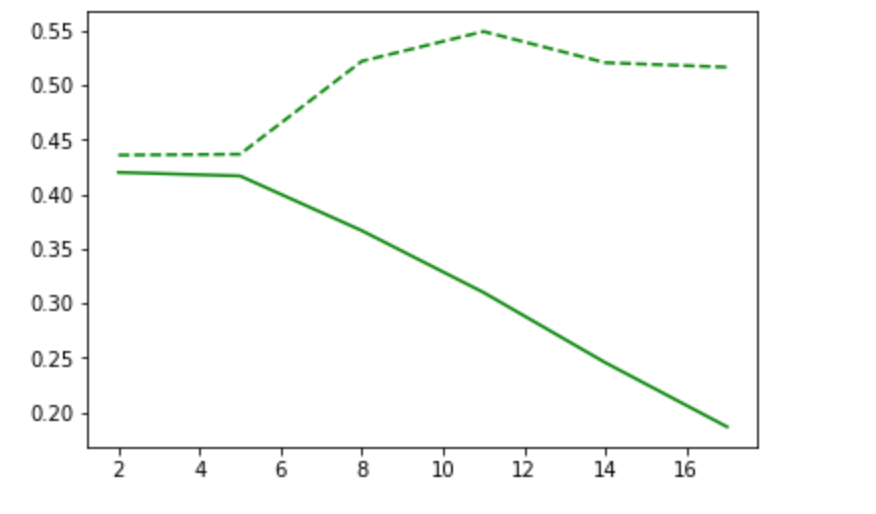
\includegraphics[width=8cm]{figure/tme1/02ap.png} 
	 \caption{Taux d'erreur en fonction de la profondeur pour un partitionnement avec 20\% des données en apprentissage }
	 
\end{figure}

On remarque que plus la profondeur est grande, moins l'on a d'erreur en apprentissage, comme on l'a expliqué c'est tout a fait normal puisque notre arbre va tendre à s'adapter parfaitement aux données apprises.\\Cependant on remarque que cette tendance est inversé pour l'erreur en test, qui elle augmente plus la profondeur est grande. C'est dû au sur-apprentissage des données qui a conduit notre arbre à avoir un modèle uniquement adapté aux données apprises au détriment d'un modèle plus général.\\
De même pour un partitionnement avec peu de données en apprentissage, notre modèle sous apprend ce qui conduit à plus d'erreurs dans le test.
\clearpage
\subsection{Validation croisée : sélection de modèle.}
La problématique que l'on rencontre maintenant est comment calibrer notre classifieur et nos paramètres pour éviter le sur et sous apprentissage afin d'avoir les meilleurs scores possibles.\\
On peut utiliser la méthode de la validation croisée  ou \textit{cross-validation} qui consiste à diviser nos données en $K$ blocs de données. Ces blocs servent à entrainer notre modèle, c'est à dire à apprendre sur nos données et les différents paramètres comme la profondeur de l'arbre par exemple.\\ Puis l'on garde un de ces blocs pour tester notre modèle.\\ À la fin, on sélectionne le meilleur modèle, c'est à dire celui qui a produit le moins d'erreur en test.\\ Ci dessous notre code implémenté pour la validation croisée.\\
\section{TME 2 : Estimation de denisté.}
 Les données ici sont des points d'intérêts de la région parisienne, par exemple bar, restaurants, distributeurs etc donnés à une certaine localisation. \\L'objectif de nos algorithmes était d'éstimer la densité des ces POI à différentes localisation.\\ Différentes méthodes et algorithmes ont été utilisés, comme la méthode des histogrammes et la méthode des noyaux.\\
\begin{figure}[h]
	\center
	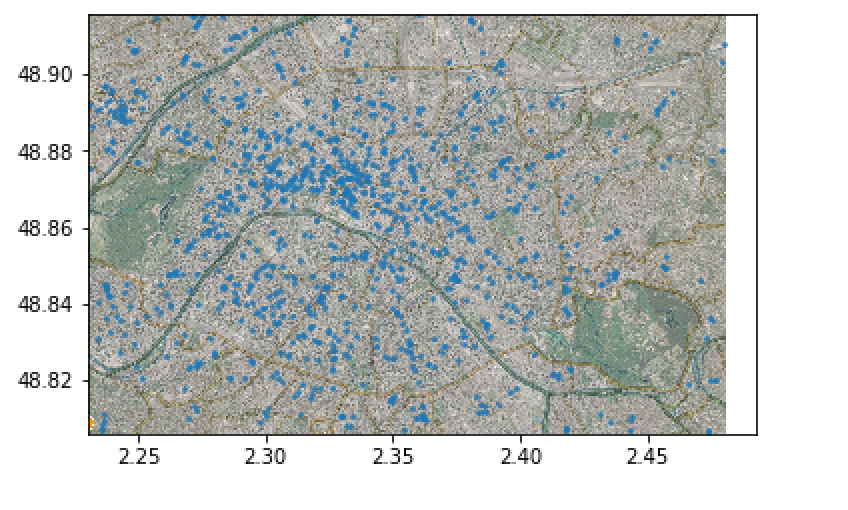
\includegraphics[width=8cm]{figure/tme2/carteATM.png} 
	 \caption{Localisation de tout les ATM à Paris et aux alentours. }
	 
\end{figure}

\subsection{Méthode des histogrammes.}
Notre premier modèle est la méthode des histogrammes, qui consiste à discrétiser notre espace puis à compter les localisations qui tombent dans chaque partis de l'espace.\\
\begin{figure}[h]
	\center
	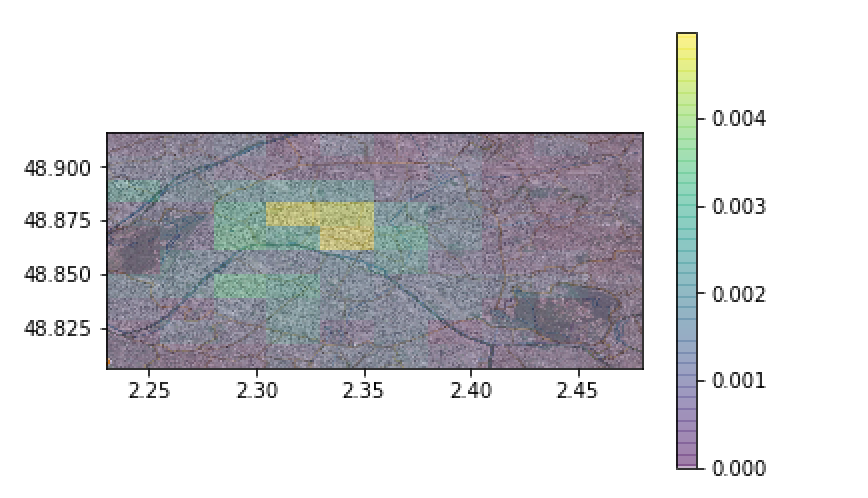
\includegraphics[width=8cm]{figure/tme2/atmHistogrammePas=5.png} 
	 \caption{Estimation de densité par histogramme sur les ATM de la Figure 5 avec un pas de discrétisation de 5. }
	 
\end{figure}
Désormais, en donnant un nouveau point on peut prédire la densité d'ATM aux alentours.

\begin{figure}[h]
	\center
	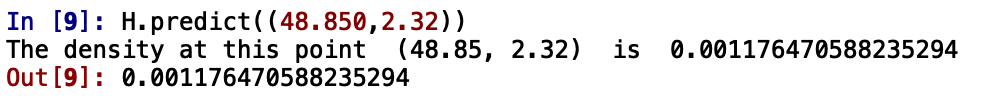
\includegraphics[width=8cm]{figure/tme2/predictHistogrammePas=5.png} 
	 \caption{Prédiction de densité sur un nouveau point avec la méthode des histogrammes. }
	 
\end{figure}
Les limites de la méthode des histogrammes sont que si l'on définit des secteurs trop grand on risque de biaiser notre estimation en attribuant la même densité à des points éloignés, ce qui n'est pas représentatif de la réalité.\\Au contraire si on définit des secteurs trop petit on aura beaucoup de zones où la densité sera nulle puisque aucun point n'est tombé dedans.\\ Pour le choix du meilleur pas de discretisation on peut également faire une $cross-validation$ sur les données.
\subsection{Méthode des noyaux.}
La méthode des noyaux permets de rectifier les problèmes de la méthode des histogrammes. \\ On a implémenté un modèle avec des noyaux de Parzen. Les paramètres du modèles sont la taille de l'hypercube $h$.

\begin{figure}[h]
	\center
	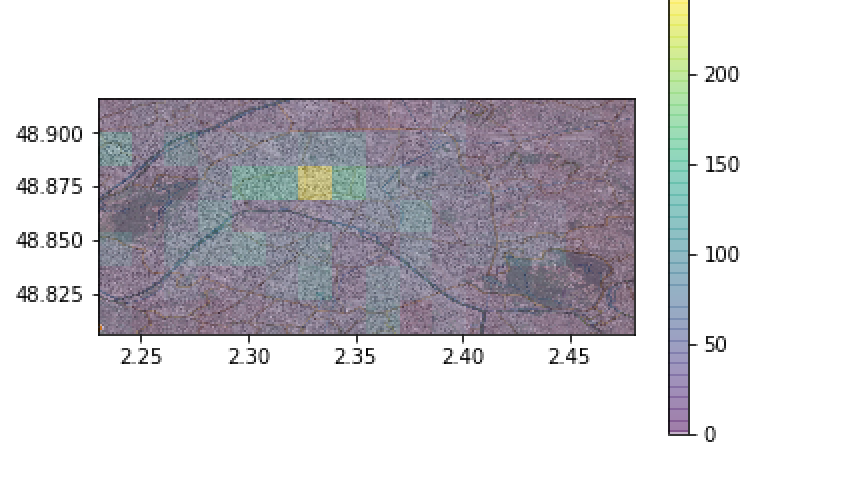
\includegraphics[width=8cm]{figure/tme2/parzenh=015.png} 
	 \caption{Estimation de densité par noyaux de Pazen sur les ATM de la Figure 5 avec $h=0.015$ }
	 
\end{figure}
On a implémenté une fonction 3D pour mieux se représenter la courbe renvoyer par les noyaux de Parzen.
\begin{figure}[h]
	\center
	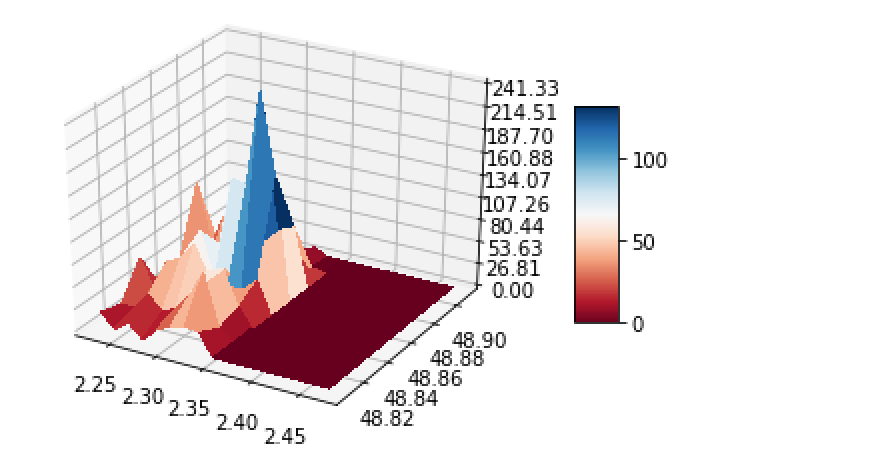
\includegraphics[width=8cm]{figure/tme2/parzen3Dh=015.png} 
	 \caption{Représentation 3D sur les noyaux de Pazen sur les ATM de la Figure 5 avec $h=0.015$ }
	 
\end{figure}
Lorsque notre fenêtre est trop petite, notre fonction va ressembler de plus en plus à des pics de Dirac, tandis que si la fenêtre est trop grande on va avoir une fonction assez uniforme.
\begin{figure}[h]
	\center
	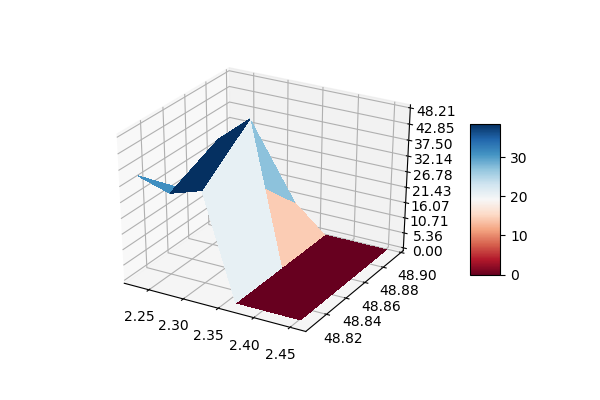
\includegraphics[width=8cm]{../tme2/parzen3Dh=045.png} 
	 \caption{Représentation 3D plutôt uniforme sur les noyaux de Pazen sur les ATM de la Figure 5 avec $h=0.045$ }
	 
\end{figure}
\begin{figure}[h]
	\center
	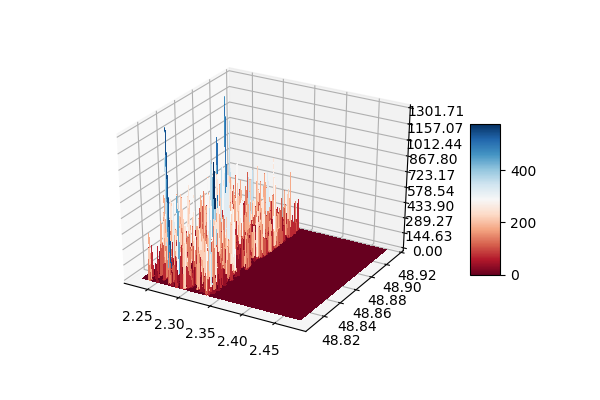
\includegraphics[width=8cm]{../tme2/parzen3Dh=001.png} 
	 \caption{Représentation 3D pic de Dirac sur les noyaux de Pazen sur les ATM de la Figure 5 avec $h=0.001$ }
	 
\end{figure}
\\
Comme pour la méthode des histogrammes on peut utiliser de la $cross validation$ pour déterminer la meilleure fenêtre possible de notre modèle.
\clearpage
\section{TME 3 : Descente de gradient.}
Dans ce TME nous nous intéressons à la descente de gradient pour optimiser des fonctions simple pour commencer, puis des fonctions qui ne sont plus optimisable analytiquement, comme dans le cas dans une regression logistique.
\subsection{Optimisation de fonctions}
Pour débuter avec des fonctions simple nous avons codé la fonction $f(x) = x\cos x$ et sa dérivé $f'(x) = \cos x - x\sin x$.\\
On voie bien sur la figure suivante que que le gradient en bleu tend vers 0 a mesure que $f$ converge vers un minimum local.\\
\begin{figure}[h]
	\center
	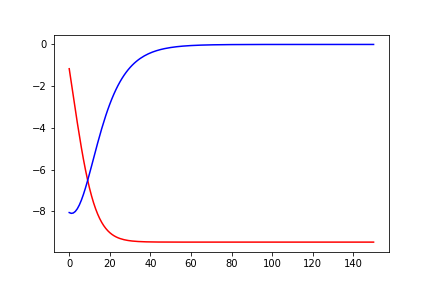
\includegraphics[width=8cm]{figure/tme3/xcox.png} 
	 \caption{valeurs de $f$ en rouge, et du gradient de $f$ en bleu, avec 150 iteration.}
	 
\end{figure}
On constate la même chose avec la fonction $f(x) = -\log x + x^2$ qui a pour dérivé $f'(x) = -\frac{1}{x}+2x $
\begin{figure}[h]
	\center
	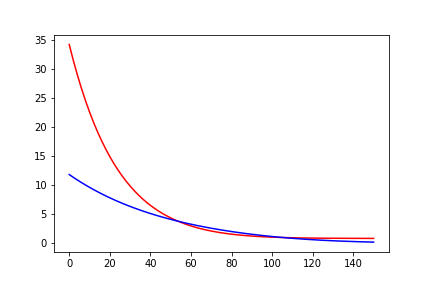
\includegraphics[width=8cm]{figure/tme3/logx.png} 
	 \caption{valeurs de $f$ en rouge, et du gradient de $f$ en bleu, avec 150 iteration.}
	 
\end{figure}
En ce qui conserne la fonction de Rosenbrock, on peux essayer de visualiser directement grace aux isocourbes ou bien à l'aide d'une projection en 3D de l'espace d'optimisation.\\
\begin{figure}[h]
	\center
	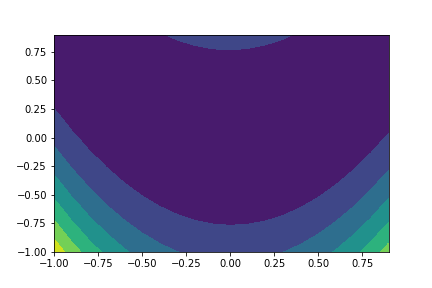
\includegraphics[width=8cm]{figure/tme3/rosenBrock2D.png} 
	 \caption{Isocourbe de la fonction de coût de Rosenbock.}
	 
\end{figure}
\begin{figure}[h]
	\center
	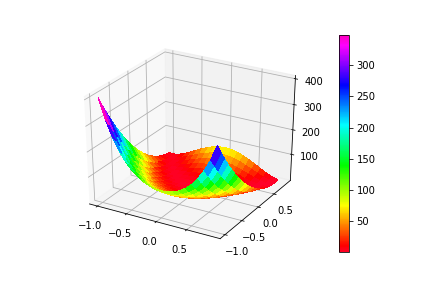
\includegraphics[width=8cm]{figure/tme3/rosenBrock3D.png} 
	 \caption{Représentation 3D de l'espace de la fonction de Rosenbock.}
	 
\end{figure}
\clearpage
\subsection{Régression logistique}
On va teste la classe 1 contre la classe 5 du jeu de données USPS pour la suite du TME. Aprés avoir entrainer le modèle, on observe un taux de 94,6\% de bonne classification sur notre jeu de données. Ce qui est plus faible qu'avec un classificateur bayésien naïf (celui de scikit learn), avec lequel on obtient 99\% de bonne classification. Toute fois il ne faut pas perdre a l'esprit que l'on a teste le score des modèles sur les mêmes données qui nous ont servie a les entraîner.\\
Pour ce que est des valeurs de w, elles sont extrement proche de 0, puisqu'elles sont compris dans un intervales allant de 0.004 à -0.002.\\
\section{TME 4 : Perceptron.}
Dans ce TME on étudie plusieurs fonctions de coût qu'on adapte à l'algorithme du Perceptron. En particulier la fonction de coût des moindres carrés et $Hing\_loss$.\\
Pour minimiser l'erreur on utilise la descente de gradient comme méthode d'optimisation qu'on implémente pour chaque fonction de coût.\\
\subsection{Données générées artificellement}
Les données sont générées artificiellement selon deux ou quatres gaussiennes. Nos modèles sont évalués sur un ensemble de train et test.\\
\begin{figure}[h]
	\center
	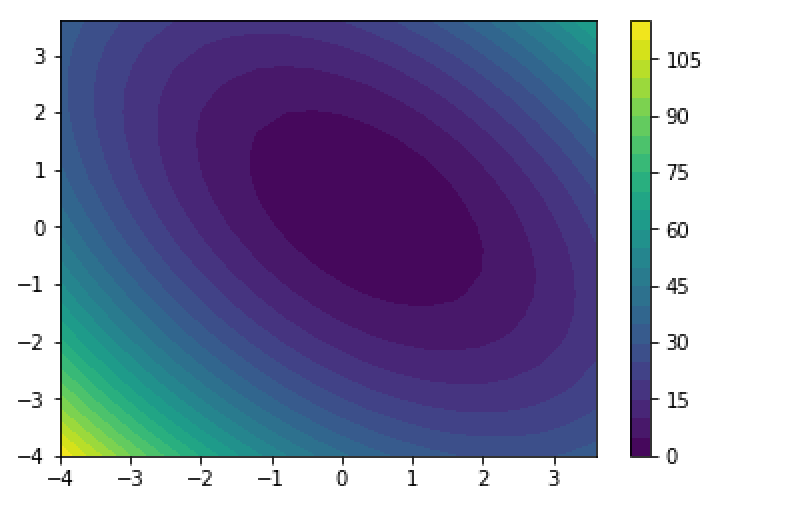
\includegraphics[width=8cm]{figure/tme4_5/mse.png} 
	 \caption{Isocourbe de la fonction de coût des moindres carrés. }
	 
\end{figure}
\begin{figure}[h]
	\center
	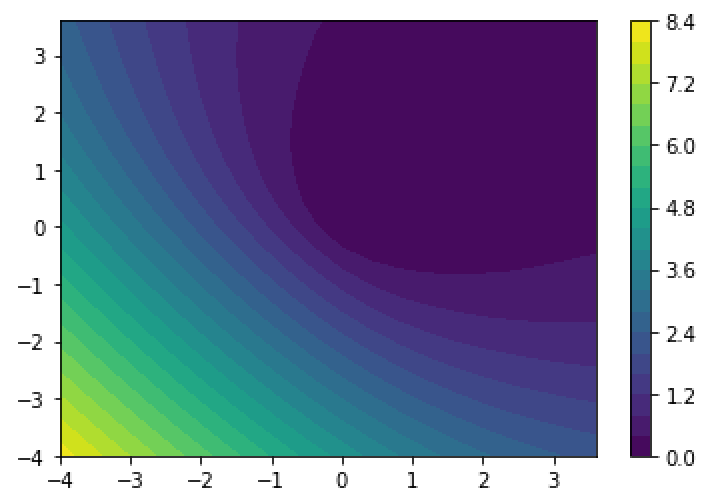
\includegraphics[width=8cm]{figure/tme4_5/hinge_loss.png} 
	 \caption{Isocourbe de la fonction de coût Hinge Loss. }
	 
\end{figure}
\begin{figure}[h]
	\center
	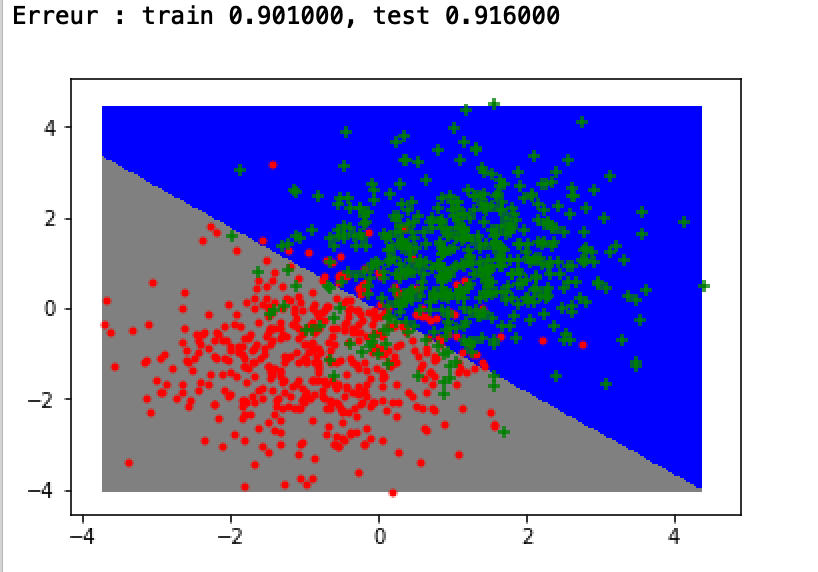
\includegraphics[width=8cm]{figure/tme4_5/borderHL.png} 
	 \caption{Score ( et non l'erreur ) du perceptron et sa frontière en utilisant Hinge Loss comme fonction de coût. }
	 
\end{figure}
\begin{figure}[h]
	\center
	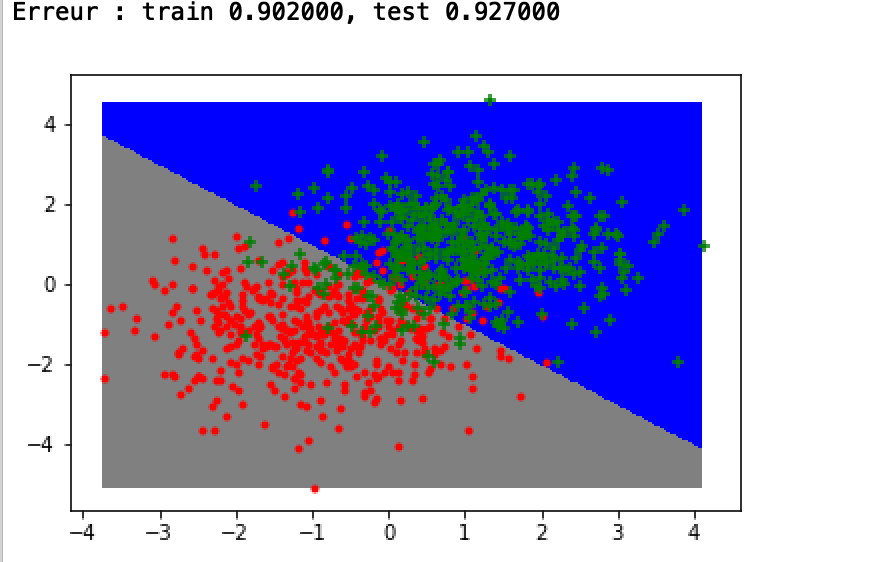
\includegraphics[width=8cm]{figure/tme4_5/borderMse.png} 
	 \caption{Score  ( et non l'erreur )  du perceptron et sa frontière en utilisant les moindres carrés comme fonction de coût. }
	 
\end{figure}
Comme la fonction Hinge Loss est une fonction convexe, l'algorithme de descente de gradient adapté à ce coût convergera forcément si l'on prend un pas $epsilon$ pas trop grand. En effet si le pas $epsilon$ est trop grand notre descente de gradient risque d'oscillé autour du minimum et de jamais l'atteindre.\\ Au contraire si notre pas $epsilon$ est trop petit notre algorithme convergera, mais lentement.\\
On remarque que les scores en apprentissage et en test des deux fonctions sont sensiblement les mêmes.\\En rajoutant une dimension à $X$ ( nos données ) qui vaut toujours 1 et maintenant dans $W$ la dernière dimension sera notre biais.\\
\clearpage
\subsection{Données USPS}
On peut utiliser l'algorithme du Perceptron pour comparer des classes entre elles, par exemple avec le fichier USPS qui contient des images scanné de chiffres écrit à la main.\\ On a implémenté une fonction qui sélectionne deux classes, c'est à dire deux nombres par exemple 1 et 7 qui sont souvent confondus, et applique l'algorithme du perceptron sur ces données pour séparer ces chiffres.\\Comme la dimension des images est de taille 256, on ne peut pas visualiser la frontière de séparation.\\

\begin{figure}[h]
	\center
	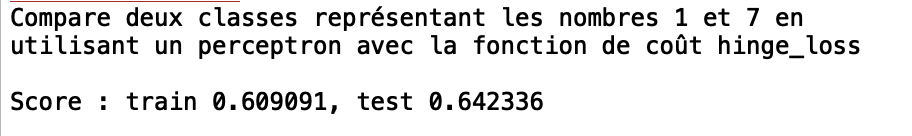
\includegraphics[width=8cm]{figure/tme4_5/compareclasse.png} 
	 \caption{Score du perceptron pour différencier les chiffres 1 et 7. }
	 
\end{figure}
Les scores en test dépassent rarement 70\% ce qui n'est pas énorme, cela peut s'expliquer puisque la frontière du perceptron en apprentissage n'est pas forcément optimale. On verra qu'avec des SVM on atteint de bien meilleur score.


\section{TME 6 : SVM et Noyaux.}
Dans ce TME nous avons étudié les Support Vector Machine. Les SVM contrairement au Perceptron nous donnent une frontière optimale en maximisant la marge entourant la frontière de décision.\\À l'aide de différent noyaux que nous avons expérimenté, les SVM permettent également de séparer de manière non linéaire des données.\\
\subsection{Données artificielles et utilisation de plusieurs noyaux.}
Sur les données générées artificiellement on a testé plusieurs noyaux pour les SVM.
\begin{figure}[h]
	\center
	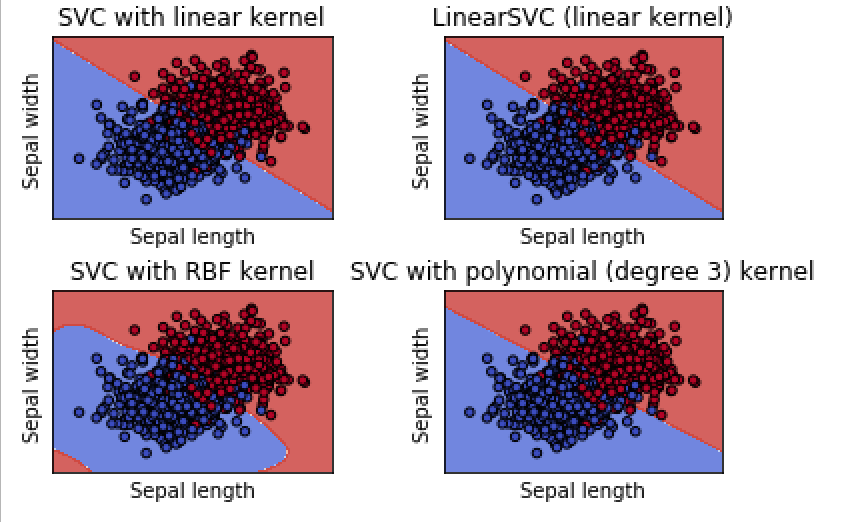
\includegraphics[width=8cm]{figure/tme6/svmarti.png} 
	 \caption{Graphique montrant les SVM avec plusieurs noyaux appliqué sur les données générées artificiellement.  }
	 
\end{figure}
\begin{figure}[h]
	\center
	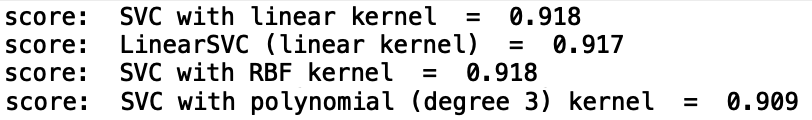
\includegraphics[width=8cm]{figure/tme6/score.png} 
	 \caption{Score des différents SVM avec plusieurs noyaux appliqué sur les données générées artificiellement. }
	 
\end{figure}
On remarque bien que certaines des frontières notamment avec un noyaux RBF ne sont pas des frontières linéaires.\\
Pour ces données nous n'obtenons pas de meilleures scores qu'avec le perceptron, c'est à dire entre 90 et 95\%. Ce n'est pas surprenant puisque ces données sont facilement séparable linéairement.
\clearpage
\subsection{Comparaison de plusieurs classes sur les données USPS.}
\subsubsection{One versus One.}
Comme pour le TME sur le Perceptron, on a essayé de comparé les classes de chiffres entre elles, et voir si avec les SVM on obtenait de meilleurs résultats.\\
\begin{figure}[h]
	\center
	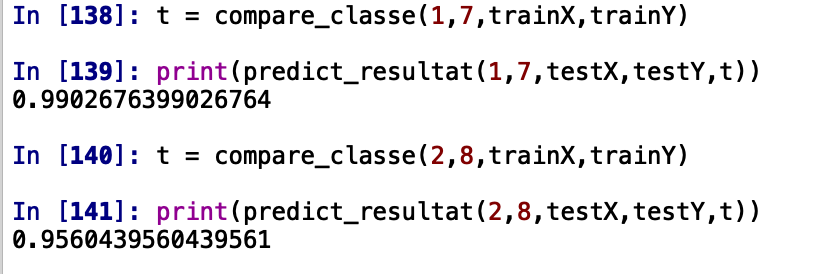
\includegraphics[width=8cm]{figure/tme6/oneversusall.png} 
	 \caption{Score pour la différentiation de deux classes avec des SVM de noyau linéaire sur les données USPS. }
	 
\end{figure}
\clearpage
\appendix
\section{Code TME ARBRES DE DÉCISION}
\verbatiminput{../tme1/tme1final.py}
\clearpage
\section{Code TME ESTIMATION DE DENSITÉ}
\textbf{On a crée un fichier Prediction.py avec nos classes pour chaque modèles.}\\
\textit{Prediction.py}
\verbatiminput{../tme2/Prediction.py}
\textit{tme2-poi.py}
\verbatiminput{../tme2/tme2-poi.py}
\clearpage
\section{Code TME3}
\verbatiminput{../tme3/tme3-etu.py}
\clearpage
\section{Code TME PERCEPTRON}
\verbatiminput{../tme4_5/tme4_etu.py}
\clearpage
\section{Code TME SVM}
\verbatiminput{../tme6/SVM.py}
\end{document}